\item \textbf{{[}YIJC/PRELIM/9569/2020/P1/Q5{]} }

YI restaurant serves a variety of local dishes at reasonable prices
and plans to provide food delivery services to its customers via a
web application. A customer places an online order and an employee
will be assigned by the system to deliver the order to the customer.
The customer can choose to pay online when ordering or make cash payment
upon delivery. Customers can choose more than one dish in the same
online order and each order has a unique ID. 

At the time of ordering, the application records the following data: 
\begin{itemize}
\item Customer name, delivery address and email, if the customer has not
placed an online order before 
\item Customer ID 
\item Order date 
\item Order time 
\item Payment mode 
\item Dish and quantity 
\end{itemize}
The following shows an example of the order receipt which will be
sent to the customer\textquoteright s email address. 
\begin{center}
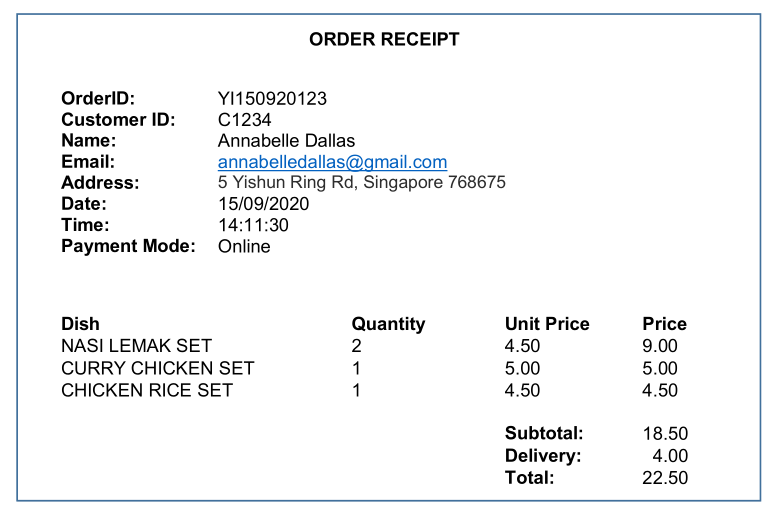
\includegraphics[width=0.5\paperwidth]{C:/Users/Admin/Desktop/Github/question_bank/LyX/static/img/9569-YIJC-2020-P1-Q5}
\par\end{center}

The restaurant assigns a unique ID to each employee and maintains
its employees\textquoteright{} information, such as their name, contact
number and bank account number. The restaurant keeps a record of the
employees\textquoteright{} delivery assignments, the date and time
when the order is successfully delivered to the customer. 
\begin{enumerate}
\item The company wants to model this application using a relational database. 
\begin{enumerate}
\item The database needs three tables to store the data for the customers\textquoteright{}
food order: \texttt{CUSTOMER}, \texttt{ORDER} and \texttt{FOOD}. 

Draw an Entity-Relationship (E-R) diagram showing the three tables
and the relationships between them. \hfill{}{[}2{]}
\item The database needs three tables to store the data for the employees\textquoteright{}
delivery assignment: \texttt{EMPLOYEE}, \texttt{ORDER} and \texttt{ASSIGNMENT}. 

Draw an Entity-Relationship (E-R) diagram showing the three tables
and the relationships between them. \hfill{}{[}2{]}
\item Draw the overall Entity-Relationship (E-R) diagram showing the five
tables and the relationships between them. \hfill{}{[}1{]}
\end{enumerate}
\item A table description can be expressed as: 

\texttt{TableName (}\texttt{\uline{Attribute1}}\texttt{, Attribute2{*},
Attribute3,...)} 

The primary key is indicated by underlining one or more attributes. 

Foreign keys are indicated using an asterisk or dashed underline. 

Write table descriptions for the five tables.\hfill{} {[}6{]}
\item Describe a method to protect data from loss or corruption.\hfill{}
{[}2{]}
\item Explain how Singapore\textquoteright s Personal Data Protection Act
(PDPA) protects the personal data of the customers and employees stored
in the database. \hfill{}{[}2{]}
\item Describe the impact of such food delivery applications on the society
and economy.\hfill{} {[}4{]}
\item With an increase in demand for food delivery, the restaurant wishes
to enhance the food delivery services to cater to the larger volume
of orders and to include more features in the application such as
real time location tracking of the food order and customers\textquoteright{}
review of the dishes, yet ensuring that the application maintains
fast performance. The restaurant is now considering using a NoSQL
DBMS instead of a relational database. 

State and explain \textbf{two} reasons why NoSQL DBMS may be more
suitable for the proposed scenario.\hfill{} {[}4{]}
\end{enumerate}